\documentclass{article}
\usepackage{authblk}
\usepackage[a4paper, total={6in, 9in}]{geometry}
\usepackage{wrapfig}
\usepackage{booktabs}
\usepackage{graphicx}
\usepackage{float}
\usepackage{apalike}
\usepackage[section]{placeins}
\usepackage[hidelinks]{hyperref}
\title{Allowances and Universal Basic Income}
\author[1]{Nikhil Woodruff}
\affil[1]{UBI Center}

\begin{document}
    \maketitle
    \begin{figure}[h]
        \href{http://www.ubicenter.org}{
\includegraphics[width=0.3\textwidth]{images/ubicenter.png}}
        \centering
        \end{figure}
    \begin{abstract}
        Under UK law, portions of income known as allowances are disregarded from taxation and benefit withdrawal. For example, the personal allowance exempts the first £12,570 of income from taxation for most individuals. Means-tested benefits have similar allowances, and some forms of income like dividends have their own tax allowances.

        I survey these allowances and, using the open-source OpenFisca UK microsimulation model, estimate the distributional effects of exchanging them for budget-neutral UBI schemes. I find that a combination of different allowance repeals could fund a universal basic income of over £2,000 per year, would be distributionally progressive and would reduce poverty. In addition, quantifying the efficiency of allowance-repeal funded UBI schemes as antipoverty poverty shows significant differences in the effectiveness of different allowances as UBI funding sources.
    \end{abstract}
    \section{Introduction}
    Allowances are sections of the tax-benefit system which disregard income for the purposes of tax and benefit calculations. Their existence often causes significant amounts of lost revenue, especially in the tax system. In this paper, I estimate the static\footnote{Static effects do not incorporate labour supply responses or the effects of changes to macroeconomic variables, instead estimating the effects of a reform immediately after its enactment} effects of replacing different allowances with budget-neutral universal basic income schemes, on the income distribution, poverty and other socioeconomic indicators. I model reforms to the UK tax-benefit system with the OpenFisca-UK microsimulation model,\footnote{Full model source code is available at \href{https://github.com/PSLmodels/openfisca-uk}{https://github.com/PSLmodels/openfisca-uk}. The source code for all results, figures and tables is available at \href{https://github.com/ubicenter/uk-allowances}{https://github.com/ubicenter/uk-allowances}.} using the Family Resources Survey uprated to 2020-21. 

    The largest potential sources of funding in this paper for UBI reforms are the Personal Allowance and the National Insurance Primary Threshold/Lower Profits Limit. The Personal Allowance represents a far-reaching tax cut and would provide the most transformative UBI policy if replaced completely. The National Insurance thresholds, for employment and self-employment income respectively, are technically distinct from allowances, due to their independence from higher thresholds. However, they are included in this paper given their similarity as a tax base-broadening funding source to the Personal Allowance. 
    
    After the main Income Tax and National Insurance allowances, repealing several other allowances would raise small amounts of revenue and simplify the tax-benefit system: the Dividend, Property and Trading allowances, and the Universal Credit Work Allowances.
    \section{Personal Allowance}
    The Personal Allowance is an allowance for most UK individuals, deductible from all forms of income for Income Tax. It is the largest and fastest-growing allowance in the tax code, with most of its gains seen during the Coalition government of 2010-2015, currently standing at £12,570 per year. Figure \ref{fig:PA_hist} shows historical levels of Income Tax allowances; only the Blind Person's Allowance has remained as consistent a component of the tax system.
    \begin{figure}
        \centering
        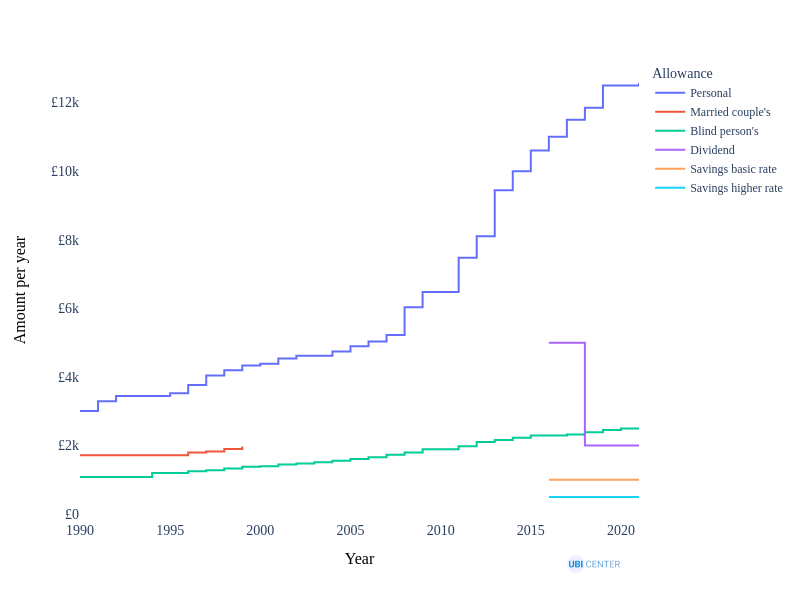
\includegraphics[width=0.8\textwidth]{images/fig_1.png}
        \caption{Historical allowance levels}
        \label{fig:PA_hist}
    \end{figure}

    \subsection{Current System}

    \paragraph{Effects on income}

    From its effect on taxable income, the Personal Allowance significantly decreases Income Tax revenue. Using the OpenFisca-UK microsimulation model, I estimate allowance reduces income tax revenue approximately £105.9bn in 2020. However, this does not equal the net revenue raised by its abolition - the Personal Allowance, by increasing post-tax income, reduces necessary welfare spending. For example, for each £1 increase in post-tax income for an individual on the Universal Credit taper, the benefit amount is decreased by 63p. 
    
    Conversely, decreasing the individual's post-tax income by reducing the Personal Allowance would necessitate increases in total government spending on means-tested welfare benefits. I estimate that, after taking increases in benefit spending into account, abolishing the Personal Allowance per year would raise £98.3bn per year.
    
    \paragraph{Margin effects} Figure \ref{fig:PA_mtr_effects} shows the changing effective marginal tax rate (the negative tax and benefit response to net income after taxes and benefits for every £1 of employment income) over the income spectrum for a hypothetical individual\footnote{For this example (a single person with no children), we assume the individual claims all benefits to which they are eligible and pays all taxes for which they are liable.}. 
    
    The Personal Allowance applies to the vast majority of UK individuals, but some are excluded by the use of means-testing: individuals with an adjusted net income (taxable income) of over £100,000 begin to see their Personal Allowance phased out at a rate of 50\% as they increase taxable income. This increases tax revenue, but creates a period of higher marginal tax rates for earnings in the region, reaching an effective marginal tax rate of 60\% for the income range between £100,000 and £125,000.

    \begin{figure}
        \centering
        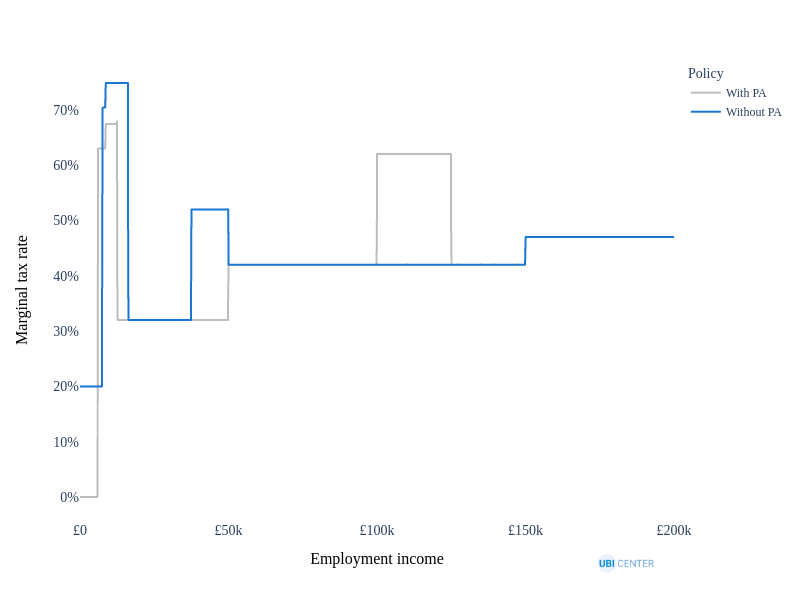
\includegraphics[width=0.8\textwidth]{images/fig_2.png}
        \caption{Marginal tax rate effects of the Personal Allowance}
        \label{fig:PA_mtr_effects}
    \end{figure}
    
    The Personal Allowance also reduces marginal tax rates at the lower end of the income spectrum, but the effect is smaller than 20\% as reductions in tax MTRs are partially offset by increases in benefit phaseout. The allowance shortens the region of punitively high effective marginal tax rates caused by benefit withdrawal by this effect, and its synchronisation with the National Insurance Upper Earnings Limit avoids a sharp increase in marginal tax rates shortly for middle-income earners.

    \begin{figure}
        \centering
        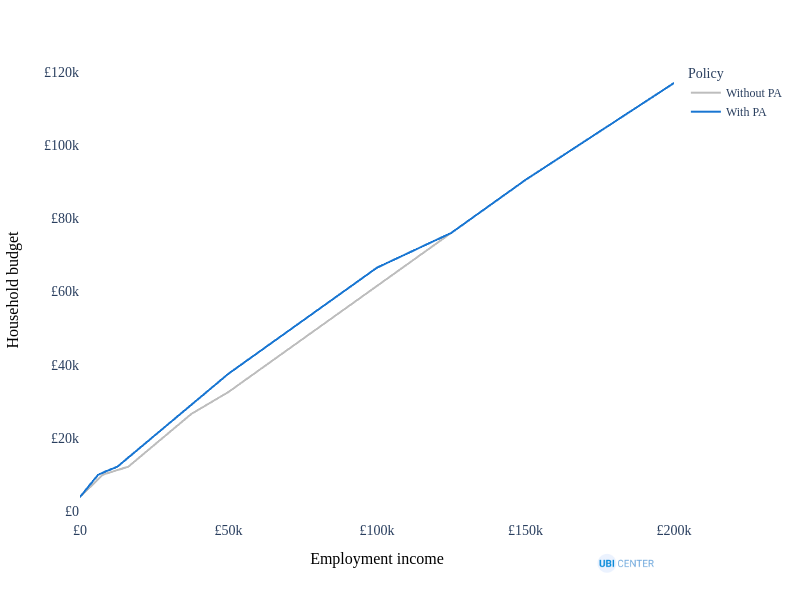
\includegraphics[width=0.8\textwidth]{images/fig_3.png}
        \caption{Budget effects of the Personal Allowance}
        \label{fig:PA_budget_effects}
    \end{figure}

    \paragraph{Budget effects} The gain seen by individuals is maximised in the higher income regions, between £50,000 and £100,000. However, its inclusion in the tax code is disproportionately beneficial in absolute amount to those on higher incomes before the phase-out (due to the fact that it effectively delays the current marginal tax rate schedule, which increases monotonically within the range of the Personal Allowance). Changes to the Personal Allowance since 2010 have benefited higher-income households more in both percentage and absolute terms.\cite{sterling_arnold} As shown by Figure \ref{fig:PA_budget_effects}, absolute financial gain increases with income (before the phase-out). 

    \subsection{UBI Replacement}

    Repealing the Personal Allowance raises a significant amount of increased tax revenue, posing the question of how the socio-economic effects of this revenue might differ if distributed as a universal basic income, rather than a tax cut. The details of such a UBI policy are simple: each adult and child citizen of the United Kingdom receives an equal payment: a share of the total available funds (maintaining budget neutrality). UBI payments are not included as income in means-tested benefits, allowing those on low incomes to receive the full benefit of the payment. Furthermore, including children in the payments from abolition of the Personal Allowance increases the antipoverty effects of the reform by effectively targeting families under the poverty line.\cite{ines} The results of such a reform are given in Table \ref{tab:PA_UBI_results}.
    \begin{table}
        \centering
        \begin{tabular}{llll}
\toprule
        &        & Absolute & Relative \\
Category & Metric &          &          \\
\midrule
Distributional & Gini coefficient &    -0.00 &    -4.10 \\
        & P90/P10 &   -62.49 &   -11.14 \\
        & Top 10\% share &    -0.01 &    -1.89 \\
Poverty & Overall rate (pp) &    -4.21 &   -30.93 \\
        & Deep poverty rate (pp) &    -1.12 &   -45.34 \\
        & Adult poverty rate (pp) &    -3.27 &   -30.06 \\
        & Senior poverty rate (pp) &    -0.06 &    -0.36 \\
        & Child poverty rate (pp) &   -10.34 &   -53.30 \\
        & Poverty gap (£bn) &    -7.18 &   -35.86 \\
Fiscal & Tax revenue (£bn) &   105.91 &    46.81 \\
        & Benefit spending (£bn) &   105.91 &    55.70 \\
Overall & Winners &    52.00 &        - \\
        & Losers &    47.74 &        - \\
\bottomrule
\end{tabular}

        \caption{Effects of a PA-UBI exchange}
        \label{tab:PA_UBI_results}
    \end{table}
    
    In order to provide comparability for the reforms in this paper, results are categorised in to distributional (inequality and median income), poverty (rates for specific groups and the poverty gap), fiscal (budgetary effects) and overall (percentage net winners and losers). 
    
    \paragraph{Distributional} The Gini coefficient is a measure of inequality ranging between 0 (complete equality) and 1 (maximal inequality, with all income concentrated on one entity). In these results, the Gini coefficient is calculated over the equivalised (adjusted for household composition) household disposable income for every person (adult and child) in the population. This reform reduces the Gini coefficient.
    
    \paragraph{Poverty} These results show significant reductions in poverty rates among all major demographic groups, with the strongest effects seen on child poverty. Child poverty levels are generally reduced more than others by universal basic income reforms that include children and are funded by taxation, as households with children have a lower per-capita tax liability (children mostly having no taxable income). 
    
    Figure \ref{fig:poverty_rates_hist} shows that poverty has fallen gradually over the last two decades, though not always consistently; exchanging the Personal Allowance for a UBI would outperform the absolute, before housing costs poverty rate reduction for every year in recent history.

    \begin{figure}
        \centering
        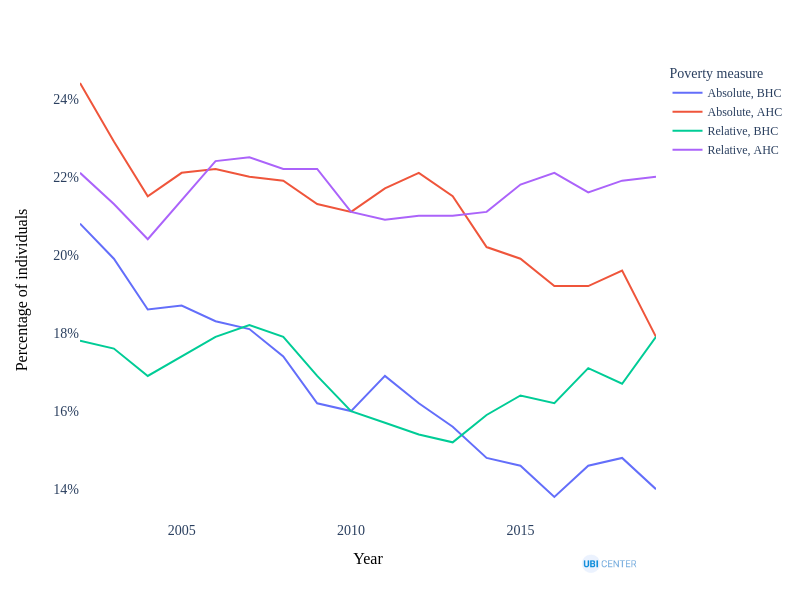
\includegraphics[width=0.8\textwidth]{images/fig_5.png}
        \caption{Historical poverty rates}
        \label{fig:poverty_rates_hist}
    \end{figure}
    
    Deep poverty is defined as living in a household whose disposable income is less than half of the poverty line. The poverty gap is the sum of the positive shortfalls between households' disposable incomes and their poverty lines - the minimum total funds required to eliminate poverty. This is a more informative measure of the poverty situation of the country, since the poverty rate does not treat separately households just below the poverty line, and those in deep poverty. This reform reduces deep poverty by 45\% and the poverty gap by 36\%.

    \section{Primary Threshold and Lower Profits Limit}

    The National Insurance Primary Threshold and Lower Profits Limit are a tax elements which remove sections of employment and self-employment income, respectively, from the tax base. Abolishing them would raise taxes on earned income, and can serve as an alternative or complementary funding method for universal basic income to abolishing the Personal Allowance.

    \subsection{Current System}
    National Insurance, separate to Income Tax, is a tax on employment and self-employment income for individuals under State Pension Age. It consists of four separate classes: Class 1, on employment income for both employees and employers; Class 2, a flat rate on self-employment income; Class 3, voluntary contributions to maintain access to associated benefits; and Class 4, a marginal rate on self-employment income.

    Defined within Class 1 are Primary (employee-side) and Secondary (employer-side) contributions, in addition to Class 1A and 1B rates, paid by employers on expenses and benefits paid to employees. Thresholds are technically distinct from allowances: reducing an allowance lowers thresholds above it, whereas reducing thresholds does not affect higher thresholds. We still consider the abolition of the lowest NI thresholds in this paper due to their similarity as a tax base-widening mechanism. 

    \begin{figure}
        \centering
        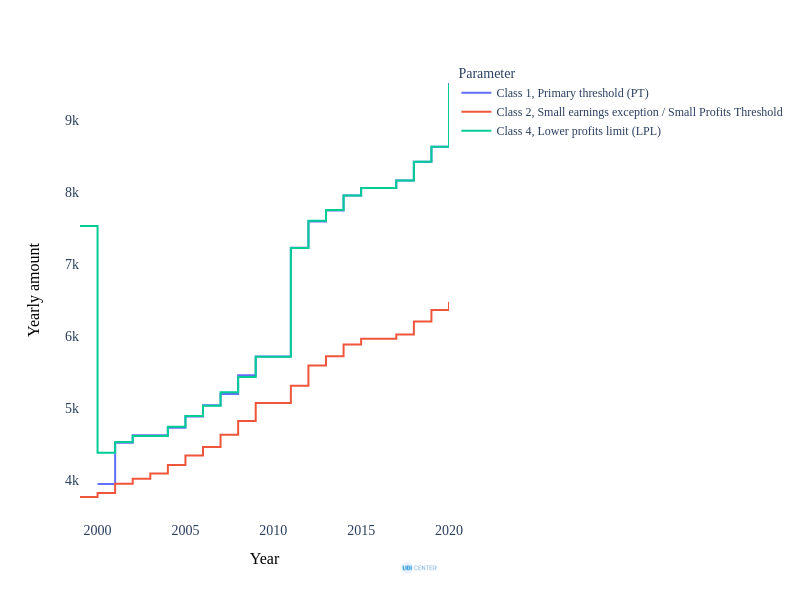
\includegraphics[width=0.8\textwidth]{images/fig_6.png}
        \caption{Historical NI thresholds}
        \label{fig:NI_thresholds}
    \end{figure}

    Shown in Figures \ref{fig:NI_thresholds} and \ref{fig:NI_rates}, thresholds and rates have risen monotonically since at least 2003. The fastest rise in thresholds took place during 2011, when the Primary Threshold and Lower Profits Limit were raised by over £1,000 per year. Rises since then have been consistent, with an increase for 2021.
    
    \begin{figure}
        \centering
        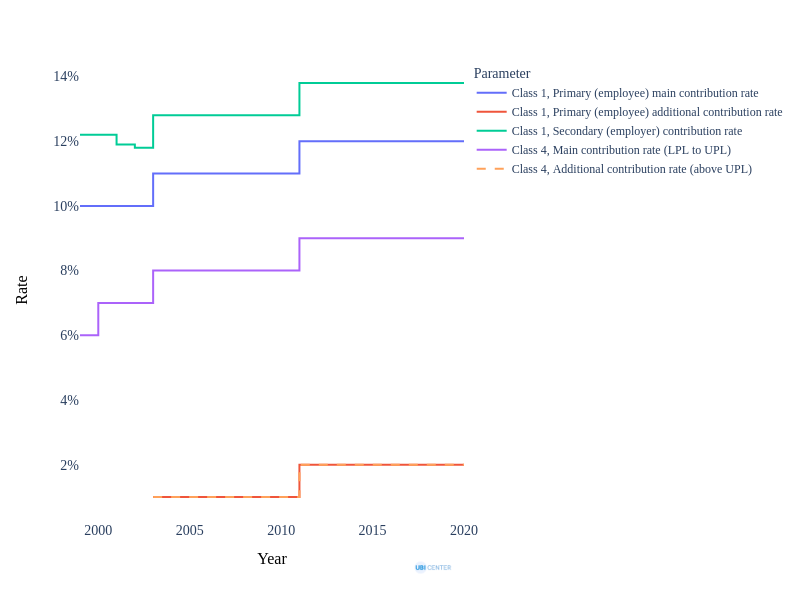
\includegraphics[width=0.8\textwidth]{images/fig_7.png}
        \caption{Historical NI rates}
        \label{fig:NI_rates}
    \end{figure}

    Rates have largely remained consistent since 2003, with a one-point rise in all rates by the Labour governments during 2003 and 2011, to fund increased health expenditure.

    \paragraph{Self-employment} The current system provides a lower tax burden for the self-employed - NI (and total tax) contributions are lower at most points in the income spectrum, except for a region caused by the flat rate of Class 2 contributions. The difference between employed and self-employed earnings taxation is primarily caused by the reduced main rate of 9\% for the self-employed, compared to 12\% for employees. 
    
    This also makes no assumption about how employer contributions affect employee pay, which would widen the gap further between employment and self-employment tax treatment. Since this paper only considers allowance and threshold reductions to fund UBI expenditure, this treatment difference, which can only be removed by equalising the main rates of National Insurance, is unchanged by the UBI reform.

    \begin{figure}
        \centering
        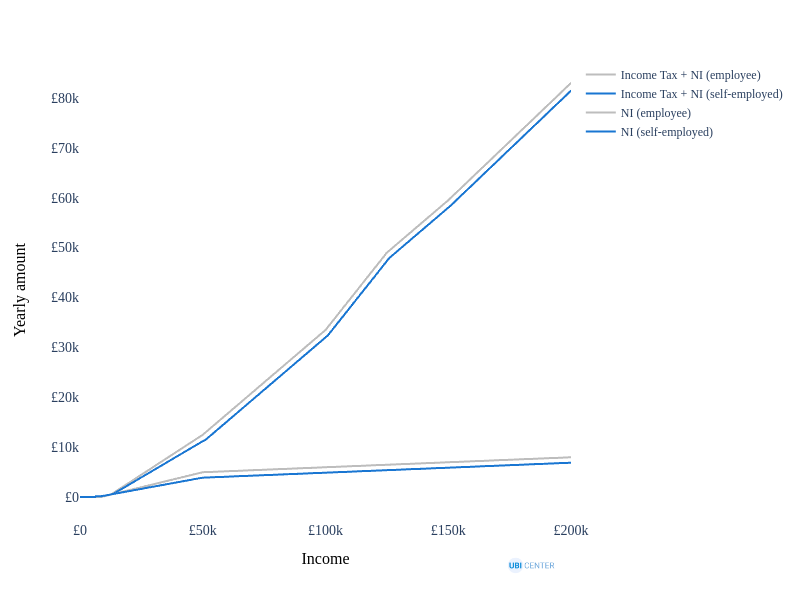
\includegraphics[width=0.8\textwidth]{images/fig_8.png}
        \caption{NI contributions for the employed and self-employed}
        \label{fig:NI_self_emp_diff}
    \end{figure}

    \paragraph{Margin effects} The PT/LPL tax reliefs do not change effective marginal tax rates as strongly as the Personal Allowance, due to the fact that National Insurance imposes much lower tax rates than Income Tax. There are, however, some changes for low-income earners, shown in Figure \ref{fig:NI_mtr_effects}: the allowance eliminates effective MTRs at earnings close to zero and transitions individuals off means-tested benefits earlier than without the allowance. This is due to individuals' applicable income for benefit programs being higher with the tax cut caused by the Primary Threshold and Lower Earnings Limit.

    \paragraph{Benefit considerations} Unlike Income Tax, National Insurance payment histories affect the payment of benefits such as the State Pension, contribution-based Jobseeker's Allowance or contribution-based Employment and Support Allowance. These programs require individuals to have a record of National Insurance payments, using specific, lower thresholds such as the Lower Earnings Limit (£120/week in 2021): individuals who earn above this threshold qualify for the benefits tied to National Insurance history. Tax reforms that remove these requirements of align the differences between employees and self-employed individuals in their entitlement based on payments are out of the scope of this paper, and therefore no change to this system is modeled.

    \begin{figure}
        \centering
        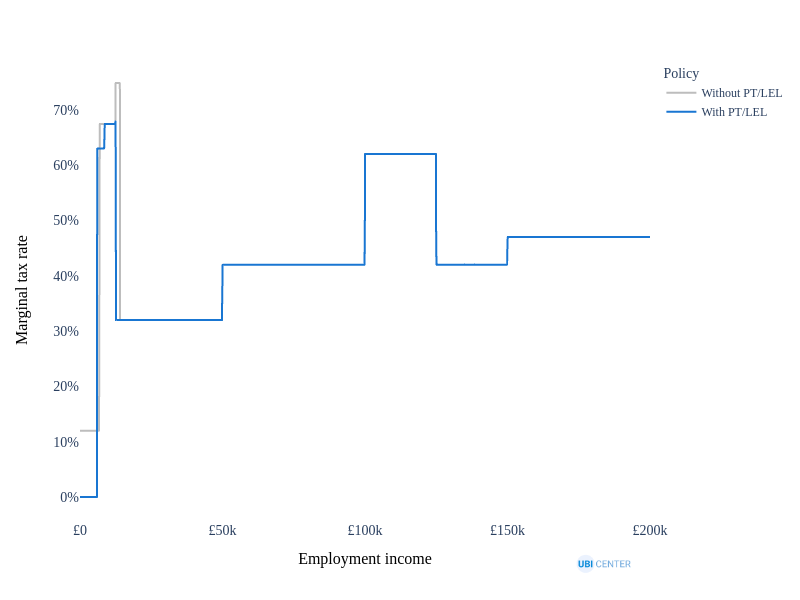
\includegraphics[width=0.8\textwidth]{images/fig_9.png}
        \caption{Effective marginal tax rate changes from the NI allowances}
        \label{fig:NI_mtr_effects}
    \end{figure}

    \subsection{UBI Replacement}

    \begin{table}
        \centering
        \begin{tabular}{llll}
\toprule
        &        & Absolute & Relative \\
Category & Metric &          &          \\
\midrule
Distributional & Gini coefficient &     -0.6 &    -1.4\% \\
        & P90/P10 &     -0.3 &    -4.9\% \\
        & Top 10\% share &   -0.2pp &    -0.6\% \\
Poverty & Overall rate &   -1.4pp &   -10.3\% \\
        & Deep poverty rate &   -0.5pp &   -19.6\% \\
        & Adult poverty rate &   -0.8pp &    -7.4\% \\
        & Senior poverty rate &   -2.0pp &   -12.3\% \\
        & Child poverty rate &   -2.7pp &   -13.9\% \\
        & Poverty gap &  -£2.6bn &   -13.1\% \\
Fiscal & Tax revenue &  £29.1bn &    12.9\% \\
        & Benefit spending &  £29.1bn &    15.3\% \\
Overall & Winners &    53.3\% &       -\% \\
        & Losers &    46.3\% &       -\% \\
\bottomrule
\end{tabular}

        \caption{Effects of exchanging the PT and LPL for a UBI}
        \label{tab:NI_UBI_effects}
    \end{table}

    The removal of zero-rated parts of National Insurance would entail setting the Primary Threshold and the Lower Profits Limit to zero. Lowering the Small Earnings Exception, above which a flat rate of £3.05 per week is mandated, is therefore not necessary. Employer-side payments are unaffected by this reform. This reform generates estimated effects shown in Table \ref{tab:NI_UBI_effects}.

    \paragraph{Distributional} Changes to National Insurance affect fewer people (only employees and the self-employed under State Pension Age), and for those that are affected, financial effects are smaller than the repeal of the Personal Allowance. The reduction in the Gini coefficient is lower. 

    \paragraph{Poverty} Poverty effects are smaller than the Personal Allowance-funded UBI overall and for children and working-age adults, but those over State Pension Age see a tangible reduction in the poverty rate, of around 12.3\%. This is expected, given that few senior citizens will be affected by the tax rises.\footnote{Few, but some are affected: while individuals of State Pension Age are not liable for National Insurance, their poverty status can still be altered if they live in a household close to the poverty line with any other person who is liable for NI.} Where repealing the Personal Allowance to fund a UBI provided only a very marginal 0.5\% reduction in senior poverty (due to the taxable status of the State Pension), the results here suggest that increases to NI contributions by widening the tax base can ameliorate some of the negative impact of Income Tax rises faced by pensioners.
    \paragraph{Fiscal} The revenue raised by the NI tax reforms is approximately one third as large as the repeal of the Personal Allowance, yet it still provides moderately strong antipoverty effects. This level of revenue is similar in nominal amount to main benefits such as Housing Benefit or Universal Credit.
    \paragraph{Overall} The share of individuals who come out ahead is slightly higher and the share who lose is slightly lower - reflecting a more concentrated burden on the working-age population and more distributed gains among the pensioner and child populations.

    \paragraph{Distributional comparison}

    \begin{figure}
        \centering
        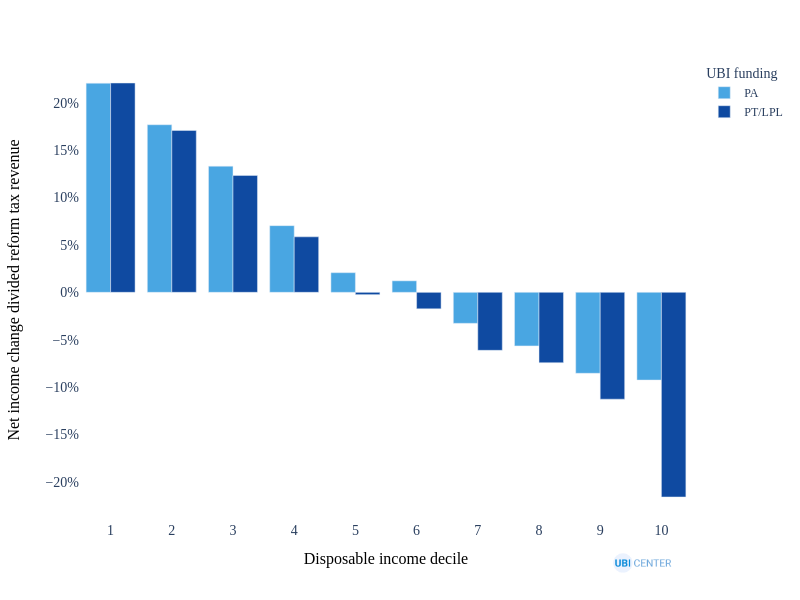
\includegraphics[width=0.8\textwidth]{images/fig_10.png}
        \caption{Share of the total UBI spending received by each decile}
        \label{fig:PA_NI_distr_comp}
    \end{figure}

    Both the Personal Allowance and the NI thresholds, exchanged for a UBI, produce progressive reforms. Figure \ref{fig:PA_NI_distr_comp} shows the share of total UBI spending received by the income deciles, making clear that while both are similar for most deciles, the National Insurance-funded UBI reform has a stronger relative impact on the top decile, due to the means testing of the Personal Allowance in the baseline system, limiting the impact of tax rises on individuals within that decile.

    \section{Smaller Allowances}

    \subsection{Current System}

    While the Personal Allowance and the National Insurance thresholds are the largest potential sources of funds for a universal basic income, other elements of the tax-benefit system could yield funding, and simplify the system. These include the Dividend Allowance, Property Allowance, Trading Allowance, and Universal Credit Work Allowances. The Dividend Allowance disregards up to £2,000 (reduced from £5,000 in 2017) of taxable dividend from taxation. The Property Allowance applies to rental income of land or property, and currently stands at £1,000 per year. The Trading Allowance currently stands at £1,000 per year, and is deductible in place of deductions for expenses from self-employment or other trading income.

    \begin{figure}
        \centering
        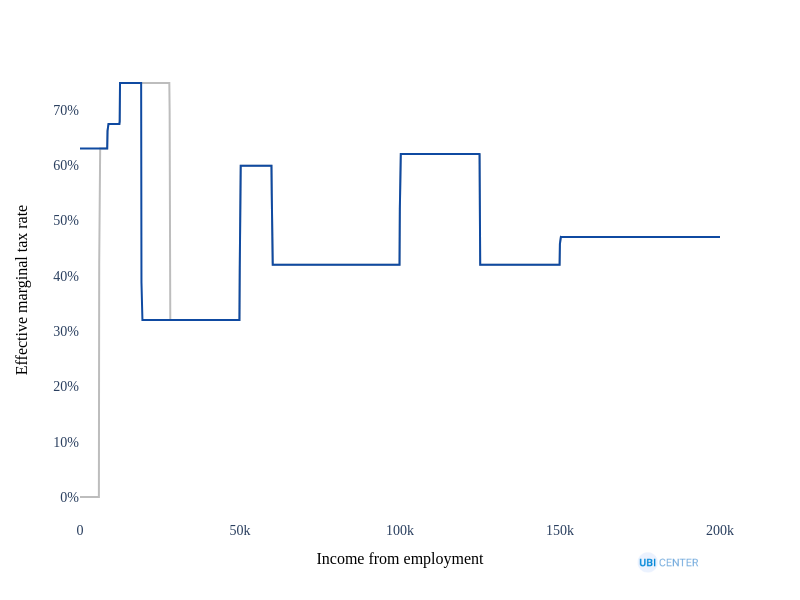
\includegraphics[width=0.8\textwidth]{images/fig_11.png}
        \caption{Change to marginal tax rates caused by lowering benefit phase-out thresholds}
        \label{fig:benefit_mtr_changes}
    \end{figure}

    The Work Allowances are disregards for earned income in benefit payment calculations, delaying benefit phase-outs beyond the allowances. I model the effects of removing the Universal Credit (UC) Work Allowance and the Tax Credit income thresholds. The UC Work Allowance varies by whether the family receives housing costs aid in their benefit payments. The current amounts are £3516 per year with housing costs aid and £6,180 per year without. The Tax Credits, now being phased out, vary the income threshold by whether the family receives only the Child Tax Credit (CTC) or both the CTC and the Working Tax Credit. Lowering the threshold of benefit phase-out raises revenue by shifting earlier the benefit reductions, maintaining the same phase-out rate (63\% on post-tax income for Universal Credit, 41\% on pre-tax income for the Tax Credits). This causes changes to the marginal tax rate landscape for individuals receiving the benefits, shown in Figure \ref{fig:benefit_mtr_changes}. 
    
    \subsection{UBI Replacement}

    Table \ref{tab:small_UBI_results} shows the relative effects of the exchange of each allowance with a UBI.

    \begin{table}[h]
        \centering
        \begin{tabular}{llllll}
\toprule
        &        & Dividends & Property & Trading &     UC \\
Category & Metric &           &          &         &        \\
\midrule
Distributional & Gini coefficient &     -0.07 &    -0.03 &   -0.03 &  -0.06 \\
        & P90/P10 &     -0.12 &    -0.03 &   -0.05 &  -0.37 \\
        & Top 10\% share &     -0.13 &    -0.09 &   -0.02 &  -0.12 \\
Poverty & Overall rate &     -0.23 &    -0.11 &    0.10 &   0.71 \\
        & Deep poverty rate &     -0.30 &    -0.21 &    0.16 &  -0.67 \\
        & Adult poverty rate &     -0.19 &    -0.16 &    0.20 &   2.73 \\
        & Senior poverty rate &     -0.38 &    -0.10 &   -0.81 &  -2.03 \\
        & Child poverty rate &     -0.20 &    -0.04 &    0.54 &  -0.75 \\
        & Poverty gap &     -0.25 &    -0.20 &   -0.16 &  -0.39 \\
Fiscal & Tax revenue &      0.45 &     0.15 &    0.26 &   0.00 \\
        & Benefit spending &      0.53 &     0.18 &    0.31 &  -0.00 \\
Overall & Winners &     79.31 &    95.02 &   88.91 &  90.83 \\
        & Losers &     20.25 &     4.54 &   10.65 &   8.73 \\
\bottomrule
\end{tabular}

        \caption{Relative effects of small allowance-UBI exchanges}
        \label{tab:small_UBI_results}
    \end{table}
    The estimated results from the abolition of small allowances are mixed, but poverty is reduced slightly by exchanging the Dividend and Property Allowances for a universal basic income, but increased by exchanging the Trading and UC Work Allowances.

    \section{Comparison}

    \subsection{Poverty efficiency}

    \begin{table}[h]
        \centering
        \begin{tabular}{lrrr}
\toprule
{} &  UBI (£/year) &  Household UBI (£/year) &  Expenditure (£bn) \\
\midrule
Property Allowance               &           5.2 &                    12.2 &                0.3 \\
Primary Threshold \& LPL          &         418.1 &                   983.8 &               27.4 \\
Personal Allowance               &        1501.9 &                  3533.9 &               98.3 \\
Combined (excl. Work Allowances) &        1947.4 &                  4582.0 &              127.5 \\
Combined                         &        2082.6 &                  4900.1 &              136.4 \\
Dividend Allowance               &          14.0 &                    32.8 &                0.9 \\
Trading Allowance                &          10.1 &                    23.8 &                0.7 \\
Work Allowances                  &         114.3 &                   268.9 &                7.5 \\
\bottomrule
\end{tabular}

        \caption{Comparisons of all UBI reforms (summary)}
        \label{tab:comp_UBI_1}
    \end{table}

    \begin{table}[h]
        \centering
        \begin{tabular}{lrr}
\toprule
{} &  Poverty gap change (£bn) &  Poverty gap efficiency (\%) \\
\midrule
Property Allowance               &                      -0.0 &                        11.9 \\
Primary Threshold \& LPL          &                      -2.6 &                         9.6 \\
Personal Allowance               &                      -7.2 &                         7.3 \\
Combined (excl. Work Allowances) &                      -9.0 &                         7.1 \\
Combined                         &                      -9.2 &                         6.7 \\
Dividend Allowance               &                      -0.0 &                         5.5 \\
Trading Allowance                &                      -0.0 &                         5.0 \\
Work Allowances                  &                       0.6 &                        -8.0 \\
\bottomrule
\end{tabular}

        \caption{Comparisons of all UBI reforms (efficiency)}
        \label{tab:comp_UBI_2}
    \end{table}

    The allowances considered have significant revenue differences, but adjusting for the UBI expenditure allows for a fair comparison of their efficiency. For this, we define the \emph{poverty gap efficiency} as the reduction in the poverty gap divided by the UBI expenditure - the percentage of the reform's revenue which actually reduces poverty. Tables \ref{tab:comp_UBI_1} and \ref{tab:comp_UBI_2} show the results of each reform on this metric.
    \subsection{Distributional impact}

    \begin{figure}
        \centering
        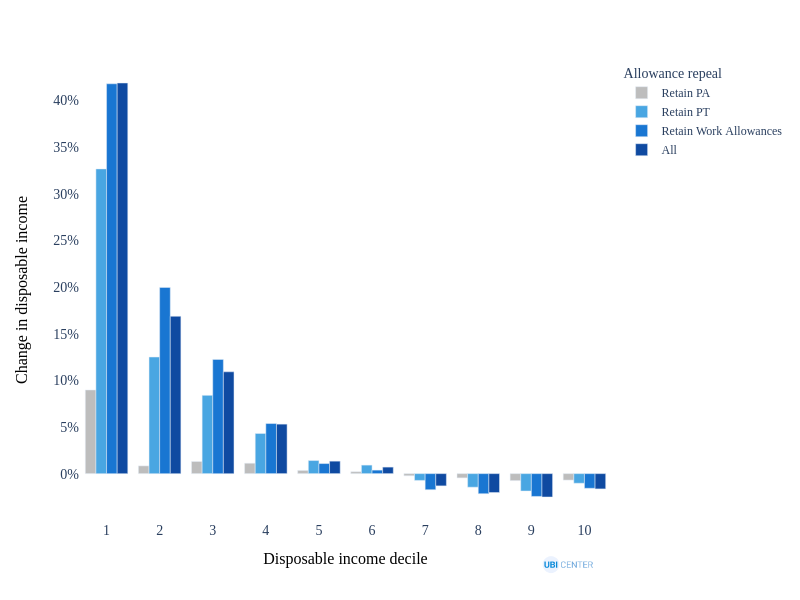
\includegraphics[width=0.8\textwidth]{images/fig_13.png}
        \caption{Distributional impacts under different funding models}
        \label{fig:distr_comp}
    \end{figure}

    Figure \ref{fig:distr_comp} shows the distributional impact of several allowance-funded UBI schemes. Starting from the combined reform abolishing all allowances considered in this paper, retaining individual allowances reduces the size of the gains or losses in disposable income deciles.  The results suggest that abolishing all considered allowances other than the Work Allowances produces the most progressive result.

    \section{Conclusion}
    The budget-neutral reforms considered in this paper would all reduce poverty and inequality, and can be combined with similar effects. The Personal Allowance provides the most significant UBI, but comes at the cost of increased risk to pension-age individuals, due to lower average incomes and the taxability of the State Pension. The National Insurance thresholds present an alternative funding method which can mitigate these effects, as well as providing additional UBI funding for increased levels of state support to individuals. Small allowances can also provide funding, though not all are equally efficient - the Property Allowance is highly efficient at reducing the poverty gap, unlike the Work Allowances.

    Universal basic income reforms require significant amounts of funding to meet their core objectives, which can be raised through many different tax or benefit policy changes. Raising tax rates on taxed income in combination with thresholding changes is often evaluated under microsimulation modeling: raising existing Income Tax rates by 5\%, reducing the Personal Allowance and raising National Insurance levels can fund a sustainable, budget-neutral UBI scheme\cite{recovery_UBI}.

    The estimated socioeconomic changes brought by the UBI reforms considered in this paper are static estimates, isolated from dynamic responses to changes in incentives provided by government taxation and spending. However, static microsimulation models can provide a level of detail on the immediate effects of a policy, and are able to estimate precise questions such as impacts on poverty levels or breakdowns of the effects of specific taxes or benefits on household budgets. UK microsimulation models such as UKMOD have facilitated in-depth analysis of a wide range of feasible basic income schemes\cite{feasible_UBI_2}\cite{feasible_UBI_1}. The estimates produced in this paper utilised OpenFisca-UK, with full source code for both the model and reforms provided for reproducibility. Microsimulation has thus far helped rapidly increase the amount of information available to the general public on the effects of policy proposals on both their individual situations and society as a whole, and the continued development of these models is critical for public understanding of universal basic income policy.

    \bibliographystyle{apalike}
    \bibliography{bib}
\end{document}